\chapter{Cơ sở lý thuyết} \label{chap:theory}
    \section{Nguyên lý hoạt động}
    Một Quadcopter gồm 4 động cơ cánh quạt gắn với nhau. Khi động cơ quay, nó sẽ tạo ra lực nâng theo phương thẳng đứng. Cánh quạt quay càng nhanh thì lực nâng càng lớn và ngược lại. Vì thế, Quadcopter có thể bay lên cao hoặc hạ xuống thấp nhờ vào sự thay đổi tốc độ quay của các cánh quạt. Để Quadcopter bay được thì tổng lực nâng tạo ra bởi 4 động cơ phải bằng hoặc lớn hơn lực hấp dẫn của Quadcopter.
    Quadcopter có thể di chuyển theo phương ngang bằng cách thay đổi lực nâng của các cặp cánh quạt. Nếu tất cả các Rotors quay theo chiều kim đồng hồ, Quadcopter sẽ bị mất kiểm soát do phản lực của momen xoắn. Để tránh trường hợp trên thì ta sẽ cho cặp cánh phía trước (front) và cặp cánh phía sau (back) quay ngược chiều kim đồng hồ, trong khi đó cặp cánh bên phải (right) và bên trái (left) lại quay cùng chiều kim đồng hồ để triệt tiêu momen xoắn.
    \begin{figure}[h!]
	        	\begin{center}
	        		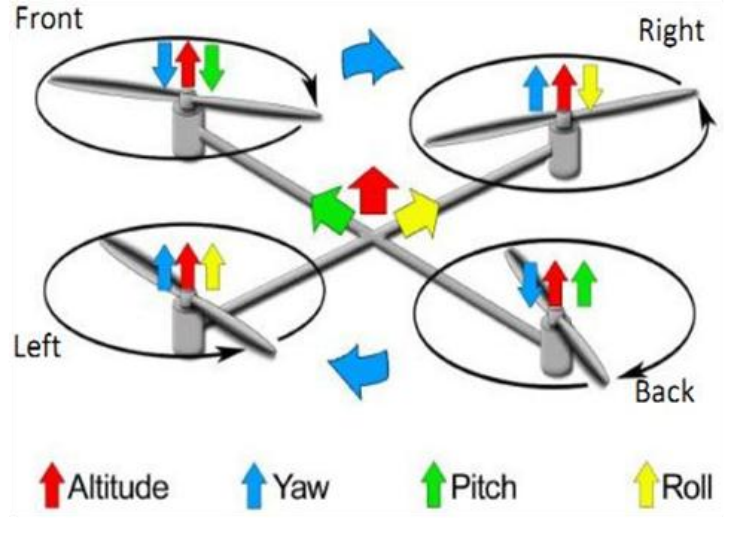
\includegraphics[scale=0.5]{images/Cuong-MoveSim.png}
	        		\caption{Chuyển động cơ bản của QuadCopter}
	        	\end{center}
        \end{figure}
        \subsection{Hệ quy chiếu}
        Quadcopter được mô hình hóa theo hệ tọa độ tham chiếu Trái Đất Phẳng. Hệ tọa độ tham chiếu Trái Đất Phẳng bỏ qua lực ly tâm và gia tốc Coriolis.
        Khung tham chiếu gồm các trục tọa độ $(x, y, z)$ là hệ thống các trục đơn giản được dùng để xác định số lượng hoặc độ lớn. Hệ trục này có thể được gắn vào thân của vật hoặc Trái Đất. Trong trường hợp này, các trục của vật $(xb,yb,zb)$ đang quay với trọng tâm là Quadcopter và các trục Trái Đất $(xe, ye, ze)$ được biểu diễn như hình.              
        \subsection{Mô hình động lực học}
        Nguyên lý hoạt động chính của mô hình này hoạt động dựa trên sự chuyển động của các dòng khí do cánh máy bay tạo ra và sự điều chỉnh vật tốc quay của cánh quạt sẽ làm thay đổi hướng bay của Quadcopter. \\
        Để mô tả chuyển động của Quadcopter ta cần 2 hệ quy chiếu:
        \begin{itemize}
        \item $e_1$ hệ quy chiếu Trái Đất.
        \item $e_B$ hệ quy chiếu khung Quadcopter.
        \end{itemize}
        \begin{figure}[h!]
        
	        	\begin{center}
	        	
	        		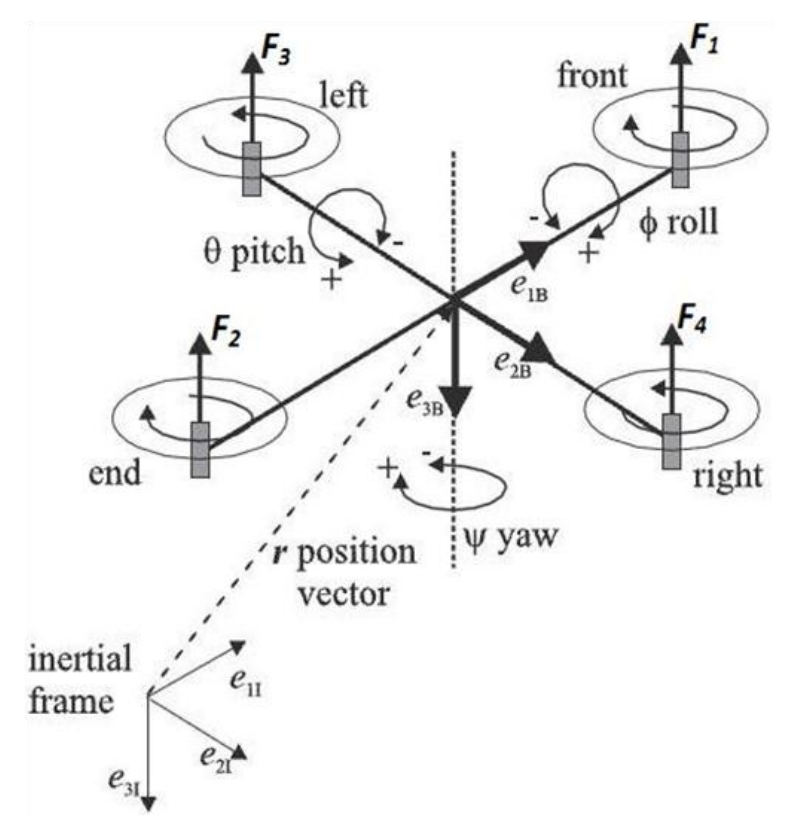
\includegraphics[scale=0.4]{images/Cuong-reference.png}
	        		\caption{Hệ quy chiếu A và B với chiều dài 1 trục L, tổng khối lượng mô hình m}
	        		
	        	\end{center}
        \end{figure}
		Sự định hướng Quadcopter được biểu thị bởi 3 góc Euler qua ma trận xoay R (2.1)
        \\
        \begin{equation}
        R=\begin{pmatrix}
c_{\psi}c_{\theta } & c_{\psi}s_{\theta }s_{\phi}-s_{\psi }c_{\theta } & c_{\psi}s_{\theta }c_{\phi}-s_{\psi }s_{\phi }\\ 
s_{\psi}c_{\theta } & s_{\psi}s_{\theta }s_{\phi}-c_{\psi }c_{\phi } & s_{\psi}s_{\theta }c_{\phi}-c_{\psi }s_{\theta }\\ 
-s_{\theta} & c_{\theta }s_{\phi} & s_{\theta }c_{\phi}
\end{pmatrix}
		\end{equation}
        Lực sinh ra của các Rotors: $F_i = b.\omega_i^2, i = 1, 2, 3, 4$ \\
       Khi đó lực nâng cho cả khung máy bay là:
        \begin{equation}
	        	T=\sum_{i=1}^{4}\left | F_{i} \right |=\sum_{i=1}^{4}\omega_{i}^{2}
        \end{equation}
        Phương trình mô tả gia tốc Quadcopter:
        \\
        \begin{equation}
        \ddot{r}=\begin{pmatrix}
\ddot{x}\\ 
\ddot{y}\\ 
\ddot{z}
\end{pmatrix}=g.\begin{pmatrix}
0\\ 
0\\ 
1
\end{pmatrix}-R\frac{T}{m}\begin{pmatrix}
0\\ 
0\\ 
1
\end{pmatrix}
        \end{equation}
        Phương trình quan hệ giữa ma trận quán tính $I_R = (I_x, I_y, I_z)$, momen quay M và momen quay hồi chuyển:
        \begin{equation}
        M_{G}:I.\ddot{\Omega}=-(\ddot{\Omega}\times I.\dot{\Omega})-M_{G}+M
        \end{equation}
        Ta có momen quay hồi chuyển phụ thuộc vào các yếu tố vận tốc xoay với $u_1 = T, u_2, u_3, u_4$ lần lượt là các đơn vị momen quay các chuyển động roll, pitch, yaw hay vận tốc quay $u^T=(u_1, u_2, u_3, u_4)$ và vận tốc góc $omega_i$ máy bay sẽ được $g(u) = w_1 + w_2 - w_3 - w_4$ (2.5)
        \\
        Kết hợp (2.5) với (2.3) và (2.4) ta có phương trình động lực học: (2.6)
        \begin{figure}[h!]
	        	\begin{center}
	        		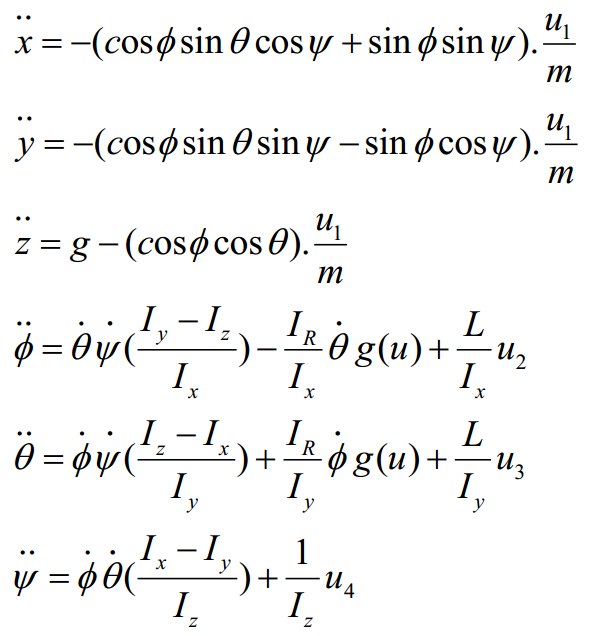
\includegraphics[scale=0.5]{images/Cuong-6.png}
	        	\end{center}
        \end{figure} 
        
        \subsection{Mô hình tính toán khí động học}
        Việc tính toán khí động học mô tả các tác động khi quay của cánh quạt trong không khí. Với các thông số $T_{MT}(N)$ là lực đẩy của cánh quạt, hướng lên, $S(m^2)$ là diện tích của cánh quạt, $\rho_{s}(kg/m^3)$ là mật độ không khí
        \\
        Ta có phương trình lực đẩy:
        \\
        $T_{MT} = 2p_sSv_1^2(N)$
        \\
        Do lực đẩy $T_{MT} = W_p = mg/4$ (trọng lượng được mang bởi một cánh quạt):
        \\
        Vận tốc dòng khí cho mỗi cánh quạt $V_1 = \sqrt{(W_p)/(2p_sS)} (m/s) $
     \section{Bộ điều khiển bay Quadcopter}
     \subsection{Thiết kế bộ điều khiển bay}
     		Bộ điều khiển phải đảm bảo rằng Quadcopter phải đáp ứng được các yêu cầu đầu vào một cách chính xác nhất. Một cấu trúc kiểm soát vòng lặp kín được sử dụng trong bộ điều khiển này vì nó sẽ làm giảm sự xáo trộn và thích nghi nhanh với bất kỳ thay đổi nào trong quá trình bay của Quadcopter. Sự phân bố trọng lượng không đều của Quadcopter cũng có thể giải quyết bằng vòng lặp kín.
            \\
            \begin{figure}[h!]
	        	\begin{center}
	        		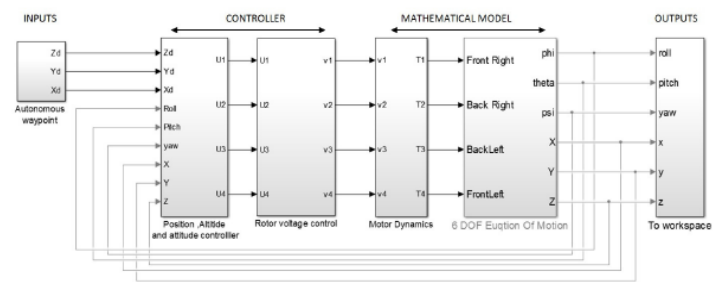
\includegraphics[scale=0.8]{images/Cuong-ModelofQc.png}
	        		\caption{Mô hình điều khiển Quadcopter}
	        	\end{center}
        \end{figure}
        	Bộ điều khiển vòng lặp kín phải đảm bảo output phải sát với input. Vòng lặp điều khiển kín là nghịch đảo của động lực Quadcopter. Khi biết được động lực của Quadcopter, bộ điều khiển sẽ được điều chỉnh và nghịch đảo của động lực Quadcopter sẽ được tính. Kết quả tín hiệu điều khiển "U" được đưa vào mô hình để cho ra output mong muốn.
            \begin{figure}[h!]
	        	\begin{center}
	        		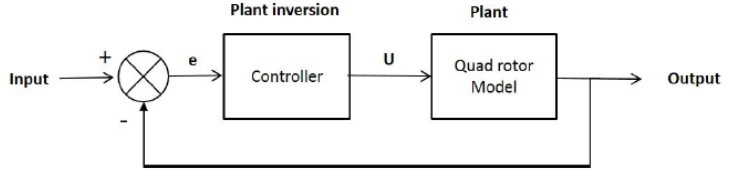
\includegraphics[scale=0.8]{images/Cuong-ClosedLoopControl.png}
	        		\caption{Mô hình điều khiển vòng lặp kín}
	        	\end{center}
        \end{figure} 
            \subsection{Nguyên lý hoạt động}
            Bộ điều khiển được xây dựng với các vòng lặp PD (Proportional Derivative). Các vòng lặp PD sẽ có trong các hành vi, độ cao và vị trí của Quadcopter để tạo ra tín hiệu điều khiển tương ứng. Quadcopter sẽ sử dụng hệ thống điều khiển PD để xác định thời gian phản hồi và giải quyết yêu cầu của nó. Bộ điều khiển PD là một hệ thống phản hồi vòng lặp kín mà nó sẽ dùng output của tín hiệu điều khiển và gửi nó vào tín hiệu input ban đầu. Ta sẽ tính toán được sự khác nhau giữa hai tín hiệu và đưa ra sự điều chỉnh. Trong trường hợp này, vị trí và hướng của Quadcopter hiện tại (tín hiệu output) sẽ được gửi đến và so sánh với vị trí và hướng mong muốn (tín hiệu input) để cho phép hệ thống điều chỉnh input và các quá trình tương ứng.
\\
			Tín hiệu sai số được thể hiện bằng công thức: $e(t) = r(t) - y(t)$
\\
			Trong đó, e(t) là tín hiệu sai số, r(t) là tín hiệu input, y(t) là tín hiệu output.
			\begin{itemize}
			\item "Điều khiển tỷ lệ" là thuật ngữ phụ thuộc vào sai số điều khiển. Nó có thể kiểm soát bất cứ phần ổn định nào. Tăng tính cân đối sẽ làm giảm thời gian phản hồi của hệ thống điều khiển. Tuy nhiên, nếu tăng tính cân đối quá cao thì hệ thống sẽ không ổn định. Phương trình cân đối: $u(t) = K_p e(t)$
\\
Trong đó, u(t) là tín hiệu input trong Quadcopter, e(t) là tín hiệu lỗi, kp là gia lượng tỷ lệ.
			\item Điều khiển dẫn xuất là khái niệm output giảm khi các biến quá trình đang tăng. Nó tác động lên tỷ lệ thay đổi lỗi. Tăng điều khiển dẫn xuất sẽ làm cho hệ thống phản hồi mạnh mẽ với các thay đổi của lỗi và tăng tốc độ phản hồi.
			\\
			$u(t) = K_dd[e(t)]/dt$
			\\
			Trong đó, Kd là hệ số đạo hàm
			\item Để xác định được giá trị của Kp và Kd, ta phải điều chỉnh bộ điều khiển cho đến khi đạt được phản hồi mong muốn. Ta dùng phương pháp Ziegler-Nichols và thủ công (trong hầu hết các trường hợp) để điều chỉnh các tỷ lệ và giá trị phát sinh. Ngoài ra, ta có thể dùng Simulink để điều chỉnh các giá trị tự động nhưng vẫn đáp ứng được yêu cầu của phản hồi.
			\end{itemize}
			\subsection{Cấu trúc bộ điều khiển}
			\begin{figure}[h!]
	        	\begin{center}
	        		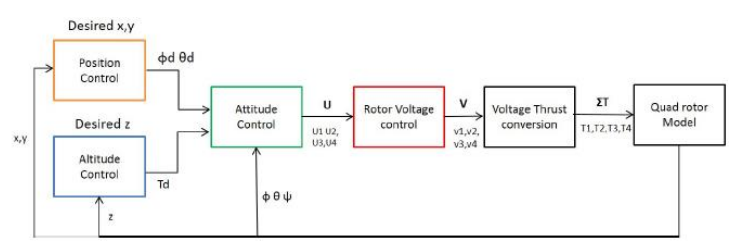
\includegraphics[scale=0.8]{images/Cuong-ControlArchitecture.png}
	        		\caption{Kiến trúc điều khiển}
	        	\end{center}
        \end{figure}
        	Các góc Roll, Pitch, Yaw được điều khiển bởi các vòng lặp PD bên trong, trong khi độ cao và vị trí được kiểm soát bởi các vòng lặp PD bên ngoài. Các vòng lặp ngoài sẽ tạo ra các giá trị mong muốn cho vòng lặp bên trong. Ta sẽ tập trung vào từng khối chi tiết trong phần sau.
\\
			\begin{itemize}
			\item Kiểm soát hành vi
			\begin{figure}[h!]
	        	\begin{center}
	        		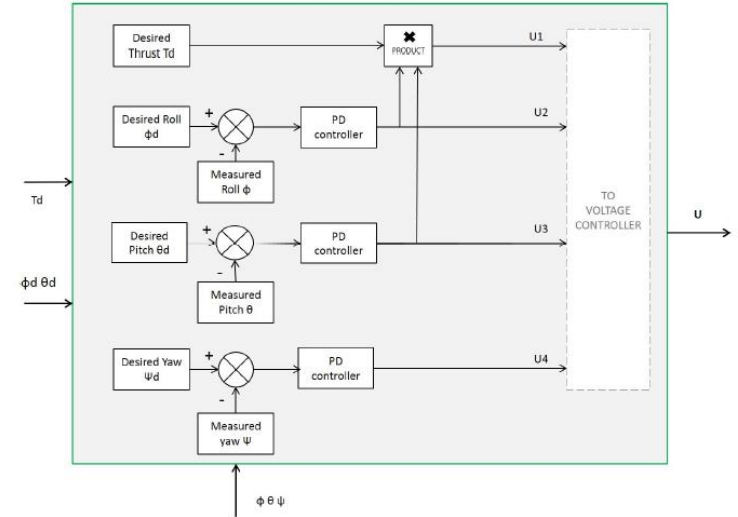
\includegraphics[scale=0.8]{images/Cuong-InnerloopIntiCon.png}
	        		\caption{Vòng lặp trong kiểm soát hành vi}
	        	\end{center}
        \end{figure}
			\\
			Vòng lặp bên trong kiểm soát các góc Roll, Pitch và Yaw. Giả sử các trục x, y của Quadcopter đối xứng, tức là điều khiển góc Pitch và Roll giống nhau. Góc Pitch giảm khi di chuyển Quadcopter về phía trước dọc theo trục X trong khi góc Roll thì di chuyển Quadcopter về bên hông.\\
			ROLL: Tín hiệu điều khiển U2 được tạo ra từ roller hoặc được truyền vào thông qua bộ điều khiển PD. Tín hiệu này sẽ điều chỉnh góc Roll của Quadcopter.\\
			PITCH: Tín hiệu điều khiển U3 được tạo ra từ pitcher hoặc được truyền vào thông qua bộ điều khiển PD. Tín hiệu này sẽ điều chỉnh độ cao của Quadcopter. Như đã nói ở trên giá trị của P và D của góc Roll và Pitch là như nhau.\\
			YAW: Tín hiệu điều khiển U4 được tạo ra từ yawer hoặc được truyền vào thông qua bộ điều khiển PD. Tín hiệu này sẽ điều khiển góc YAW của Quadcopter. Giá trị của các góc Pitch, Roll, Yaw được đo sẽ là giá trị được nạp từ output của mẫu thử.
\\
			\item Kiểm soát độ cao
			\\
			Điều khiển vòng lặp ngoài này sẽ tạo ra một lực đẩy Td để nâng Quadcopter lên độ cao mong muốn. Nó được nạp thông qua bộ điều khiển PD. Td sau đó được chuyển đến bộ điều khiển độ cao để bù trừ cho hao hụt do vector của góc Pitch và Roll. Do đó, tín hiệu điều khiển U1 sẽ giữ được độ cao mong muốn của Quadcopter mà ngay cả khi góc Roll và Pitch thay đổi. Các khối điều khiển sau sẽ cho thấy vòng lặp điều khiển và tín hiệu tương ứng bên trong bộ điều khiển độ cao. Phản hồi nhận được cung cấp độ cao của Quadcopter.
\\
\begin{figure}[h!]
	        	\begin{center}
	        		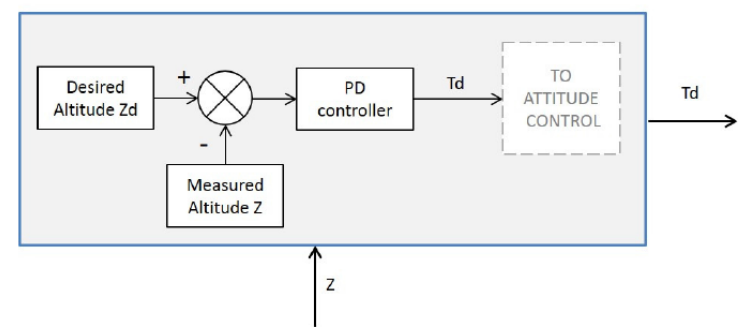
\includegraphics[scale=0.8]{images/Cuong-OuterLoop.png}
	        		\caption{Vòng lặp ngoài kiểm soát độ cao}
	        	\end{center}
        \end{figure}
			\item Kiểm soát vị trí\\
		Vòng lặp ngoài này sẽ tính toán các góc roll và pitch để đưa Quadcopter đến vị trí X và Y mong muốn. Dữ liệu phản hồi từ mô hình cung cấp giá trị X và Y. Tín hiệu vị trí sau khi tổng hợp được nạp thông qua một bộ điều khiển PD và nó tạo ra các góc Roll và Pitch mong muốn. Như đã đề cập trước đó, output của nó sẽ được nạp vào bộ điều khiển hành vi để tạo ra các tín hiệu điều khiển U2 và U3.
\\
\begin{figure}[h!]
	        	\begin{center}
	        		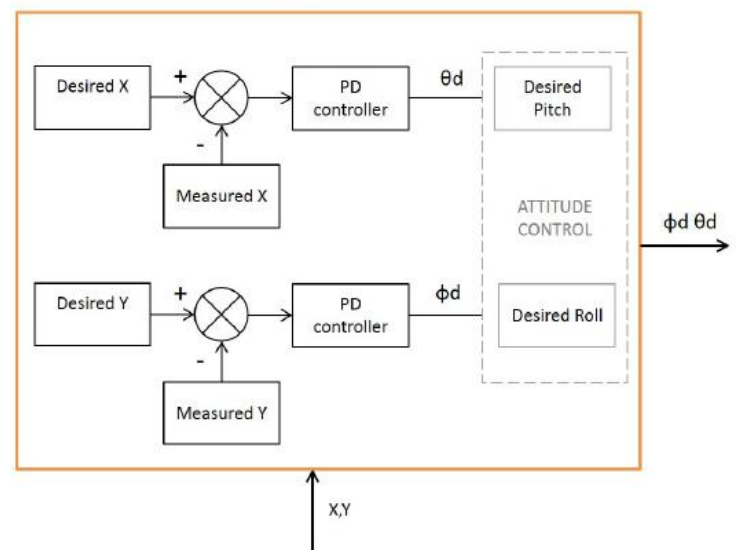
\includegraphics[scale=0.8]{images/Cuong-OuterLoopPos.png}
	        		\caption{Vòng lặp ngoài kiểm soát vị trí}
	        	\end{center}
        \end{figure}
			\item Kiểm soát điện áp của các Rotors
			\\
			Bốn inputs điều khiển được tạo ra bởi các vòng lặp trong và ngoài, nó không nạp trực tiếp vào mô hình Quadcopter vì nó là inputs lực đẩy cho bốn động cơ cánh quạt. Các tín hiệu điều khiển U được kết hơp để tạo ra tín hiệu điện áp cho mỗi Rotor. Sự kết hợp này dựa vào lực của Quadcopter để hiển thị thông số bay tương ứng. Sự kết hợp này đã được nói ở phần động cơ Rotor và được hiển thị như sơ đồ khối bên dưới. Điện áp đầu ra V sau đó được chuyển thành lực đẩy động cơ của mô hình.
  \\
  \begin{figure}[h!]
	        	\begin{center}
	        		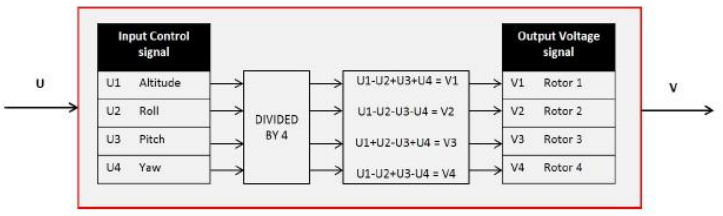
\includegraphics[scale=0.8]{images/Cuong-VolControl.png}
	        		\caption{Kiểm soát điện áp Rotors}
	        	\end{center}
        \end{figure}
			\end{itemize}
			\section{Giải thuật quadcopter theo bầy đàn}
			\subsection{Hành vi bầy đàn}
			Các Quadcopters có thể tự hoạt động theo nhiều nhóm với sự hỗ trợ của giải thuật bầy đàn. Giải thuật bầy đàn mà nhóm áp dụng thực chất là một tập hợp ba quy tắc đặc trưng của một hành vi bầy đàn đó là \textit{Gắn kết - Phân tách - Điều chỉnh} (Cohesion, Separation and Alignment).  \\
			Mỗi Quadcopter thành viên sẽ có một vùng không gian lân cận với bán kính $r_{1}$ cho trước và vùng không gian an toàn với bán kính $r_{2}$ với $r_{1}>r_{2}$. Những Quadcopters nằm trong không gian lân cận của nhau gọi là hàng xóm và khoảng cách được xác định bởi cảm biến siêu âm. Quy tắc \textit{Gắn kết} được hiểu là mỗi đơn vị sẽ tự động bay về phía vị trí trung bình của các hàng xóm của nó. 
			\begin{figure}[h!]
	        	\begin{center}
	        		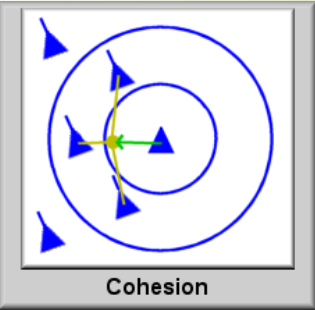
\includegraphics[scale=0.4]{images/cohesion.png}
	        		\caption{Quy tắc gắn kết}
	        	\end{center}
        \end{figure}
        \\
        Quy tắc \textit{Phân tách} giúp mỗi Quadcopter sẽ tự động tránh va chạm với hàng xóm của mình khi bị xâm nhập vào vùng không gian an toàn. Đồng thời tránh va chạm khi phát hiện có vật thể lạ nằm trong vùng lân cận.
        \begin{figure}[h!]
	        	\begin{center}
	        		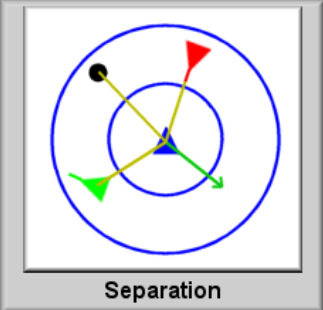
\includegraphics[scale=0.4]{images/separation.png}
	        		\caption{Quy tắc phân tách}
	        	\end{center}
        \end{figure}
        \\
        Quy tắc \textit{Điều chỉnh} giúp mỗi Quadcopter tự động bay theo hướng bay trung bình của các quadcopter hàng xóm. 
        \begin{figure}[h!]
	        	\begin{center}
	        		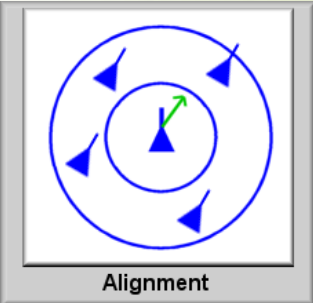
\includegraphics[scale=0.4]{images/alignment.png}
	        		\caption{Quy tắc điều chỉnh}
	        	\end{center}
        \end{figure}
        \subsection{Phương pháp Leader - Follower} 
        Với hành vi bầy đàn, các Quadcopter đã có thể tự giữ đội hình theo bầy. Sau đó áp dụng phương pháp Leader Follower chọn một Quadcopter để làm đầu đàn. Quadcopter đầu đàn sẽ là đơn vị tham khảo cho bầy. Khi ra lệnh bay cho Quadcopter đầu đàn, thông tin về vị trí của nó sẽ được xử lý bởi giải thuật bầy đàn và truyền qua cho các Quadcopter thành viên để sinh ra lệnh bay phù hợp bay theo sau con đầu đàn. 
        \begin{figure}[h!]
	        	\begin{center}
	        		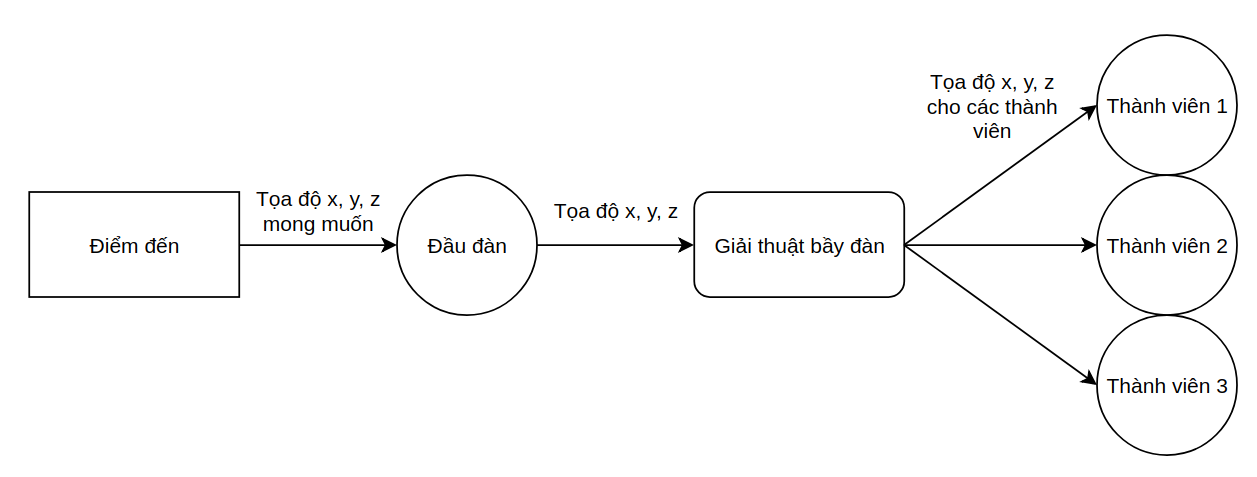
\includegraphics[scale=0.3]{images/leaderfollower.png}
	        		\caption{Mô hình Leader - Follower}
	        	\end{center}
        \end{figure}